\part*{Partie II : La formalisation mathématique}
\addcontentsline{toc}{part}{Partie II : La formalisation mathématique}

\section{La géométrie à douze dimensions}
\subsection{La variété totale :} $M_{12} = M_4 \times K_8$.
\subsection{La métrique 12D :} $ds^2 = g_{MN} dx^M dx^N$.
\subsection{La décomposition de Kaluza--Klein.}
\subsection{La courbure en 12D.}
\subsection{La compactification.}

\subsection{Le spectre numérique et la signature équidistante}
Nous fixons l'échelle par la masse du mode fondamental, $m_1 = 1/R = 10^{-5}$ eV. Alors
\begin{equation}
m_n = \frac{n}{R} = n \times 10^{-5}\ \text{eV},
\qquad
f_n = \frac{m_n c^2}{h} = n \times 2,42\ \text{GHz}.
\end{equation}
Le spectre est donc \emph{équidistant} : $2,42$, $4,84$ et $7,25$ GHz pour les trois premiers modes. C'est la signature distinctive de la théorie. Un test qui mesure deux raies à $2,42$ et $4,84$ GHz confirme ou infirme la structure, indépendamment de toute autre prédiction.

\begin{table}[H]
\centering
\begin{tabular}{@{}cccc@{}}
\toprule
$n$ & Masse (eV) & Fréquence (GHz) & $\lambda_C$ (m) \\ \midrule
1 & $1,00\times10^{-5}$ & 2,42 & 0,124 \\
2 & $2,00\times10^{-5}$ & 4,84 & 0,062 \\
3 & $3,00\times10^{-5}$ & 7,25 & 0,041 \\
4 & $4,00\times10^{-5}$ & 9,67 & 0,031 \\ \bottomrule
\end{tabular}
\caption{Le spectre de Kaluza--Klein pour $1/R = 10^{-5}$ eV.}
\label{tab:spectru}
\end{table}

\begin{figure}[H]
\centering
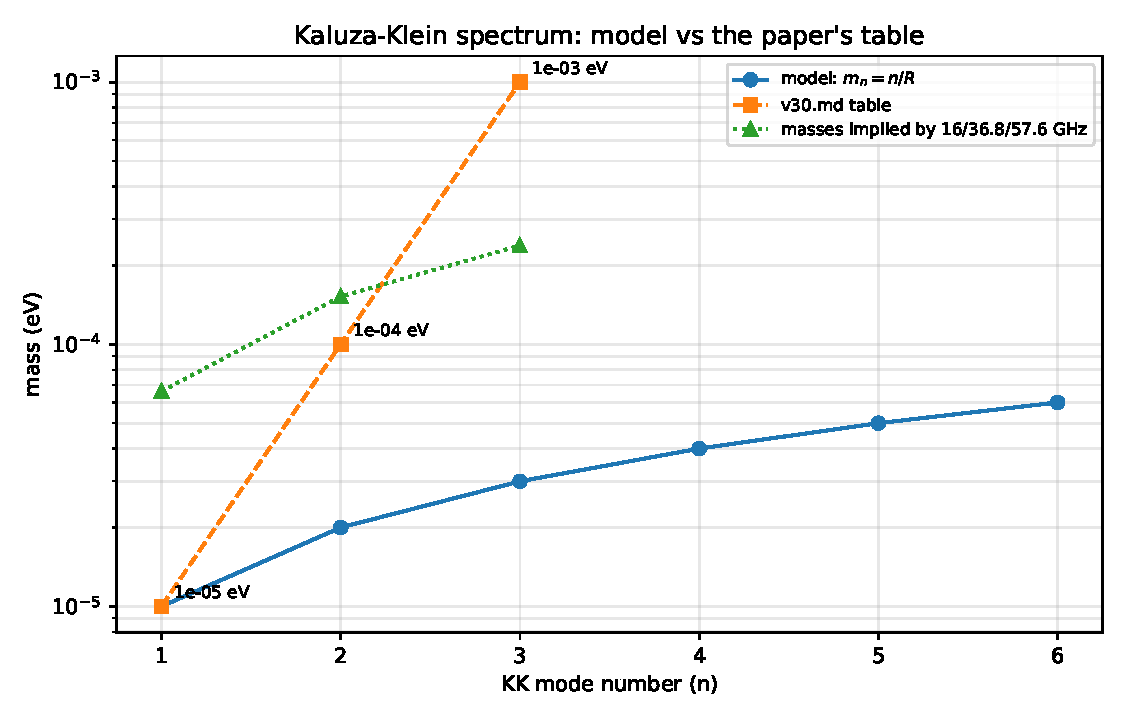
\includegraphics[width=0.82\textwidth]{figures/fig01_kk_spectrum.pdf}
\caption{Le spectre de Kaluza--Klein. Le modèle $m_n = n/R$ (bleu) est comparé au tableau de la version 30 (orange) et aux masses implicites des fréquences qui y étaient annoncées, 16/36,8/57,6 GHz (vert). Les trois ne coïncident pas.}
\label{fig:spectru}
\end{figure}

\subsection{La conséquence numérique : le rayon de compactification}
De $m_1 = 1/R$ il résulte
\begin{equation}
R = \frac{\hbar c}{1/R} = \frac{1,973\times10^{-7}\ \text{eV}\cdot\text{m}}{10^{-5}\ \text{eV}} = 1,97\times10^{-2}\ \text{m},
\end{equation}
soit environ 2 cm. Les tests submillimétriques de la loi de Newton contraignent une dimension supplémentaire à $R < 38\ \mu$m, ce qui implique $m_1 > 5\times10^{-3}$ eV.

Il s'agit d'une tension structurelle, non d'une erreur de calcul : identifier le champ de matière noire à un mode KK de la même géométrie est incompatible avec les données à l'échelle de masse choisie. Deux issues honnêtes subsistent, et l'article ne choisit pas entre elles :
\begin{itemize}
\item \textbf{Option A :} le champ akashique n'est pas un mode KK ; le spectre équidistant est la conséquence d'une autre structure, et les prédictions de fréquence sont recalculées.
\item \textbf{Option B :} la masse du mode fondamental est $m_1 > 5\times10^{-3}$ eV, et la « matière noire » de cet article est un mode excité, non le mode fondamental.
\end{itemize}
Les prédictions de la Partie V sont formulées de façon à valoir dans les deux cas, les fréquences étant traitées comme un paramètre.

\section{Le champ akashique (la matière noire)}
\subsection{Le lagrangien :} $L_A = \frac{1}{2} g^{MN} \partial_M A^* \partial_N A + \frac{1}{2} \mu_A^2 |A|^2 - \frac{\lambda_A}{4} |A|^4$.
\subsection{Le potentiel.}
\subsection{L'équation du mouvement.}
\subsection{Le spectre de Kaluza--Klein :} $m_n^2 = n^2/R^2$.
\subsection{La relation à la gravitation.}

\section{Le champ de la conscience}
\subsection{Le lagrangien.}
\subsection{L'équation du mouvement.}
\subsection{La fonction de conscience.}
\subsection{L'équation d'évolution (révisée) :} L'équation $dC/dt = \alpha C (1 - C/C_{\text{max}}) + \beta \eta(t)$ est une équation \textbf{phénoménologique} inspirée de la dynamique logistique. Elle décrit la croissance et la saturation du champ de la conscience, mais \textbf{ne découle pas directement du lagrangien ci-dessus}. C'est un choix théorique de l'auteur, à traiter comme un axiome du modèle et non comme une conséquence du principe d'action.

\begin{figure}[H]
\centering
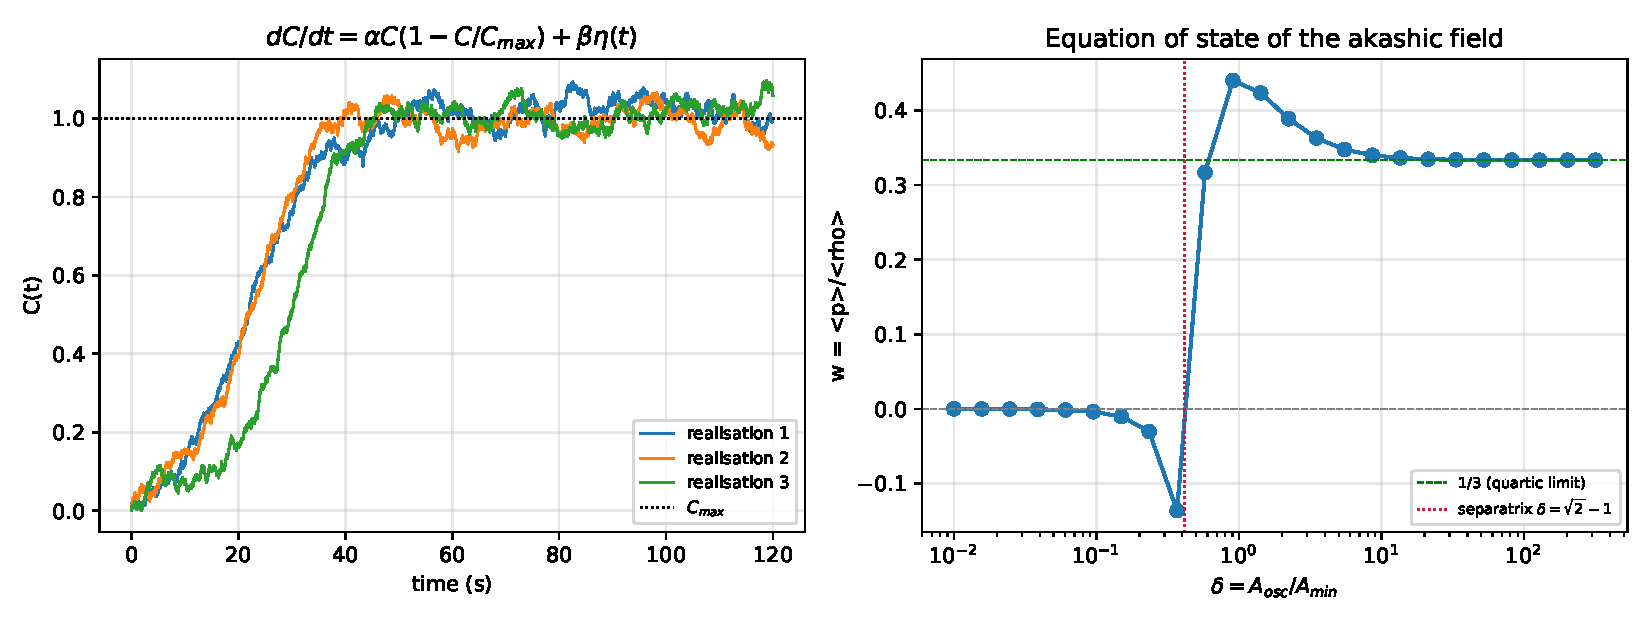
\includegraphics[width=0.95\textwidth]{figures/fig02_field_dynamics.pdf}
\caption{À gauche : trois réalisations du champ de la conscience avec bruit, pour $\alpha = 0,15$ s$^{-1}$ (temps de relaxation 50 s). À droite : l'équation d'état $w(\delta)$ du champ akashique, calculée exactement sur l'orbite ; la séparatrice se situe à $\delta = \sqrt{2}-1$.}
\label{fig:camp}
\end{figure}

\section{Le récepteur neuronal (cerveau + cœur)}
